I% Chapter Template

\chapter{Implementation and Optimizations} % Main chapter title

\label{Implementation} % Change X to a consecutive number; for referencing this chapter elsewhere, use \ref{ChapterX}

\lhead{Implementation. \emph{Implementation and optimizations}} % Change X to a consecutive number; this is for the header on each page - perhaps a shortened title

%----------------------------------------------------------------------------------------
%	SECTION - Where does time go?
%----------------------------------------------------------------------------------------

\section{Where is time spent?}

%-----------------------------------
%	SUBSECTION 1
%-----------------------------------

\subsection{Arrays}
% array creation, copy and access
% size of array argument
% system arraycopy primitive


%-----------------------------------
%	SUBSECTION 2
%-----------------------------------

\subsection{Computing indices}
% computing radix vs relaxed radix (traverse array other array)
% longer, more complex code
\[
 526843 = 00
   	 \underbracket[0.2pt][4pt]{00000}_{\text{0}}
   	 \underbracket[0.2pt][4pt]{00000}_{\text{0}}
  	 \underbracket[0.2pt][4pt]{10000}_{\text{16}}
 	 \underbracket[0.2pt][4pt]{00010}_{\text{2}}
	 \underbracket[0.2pt][4pt]{01111}_{\text{15}}
     \underbracket[0.2pt][4pt]{11011}_{\text{27}}
\]

\begin{figure}[h!]
  \centering
  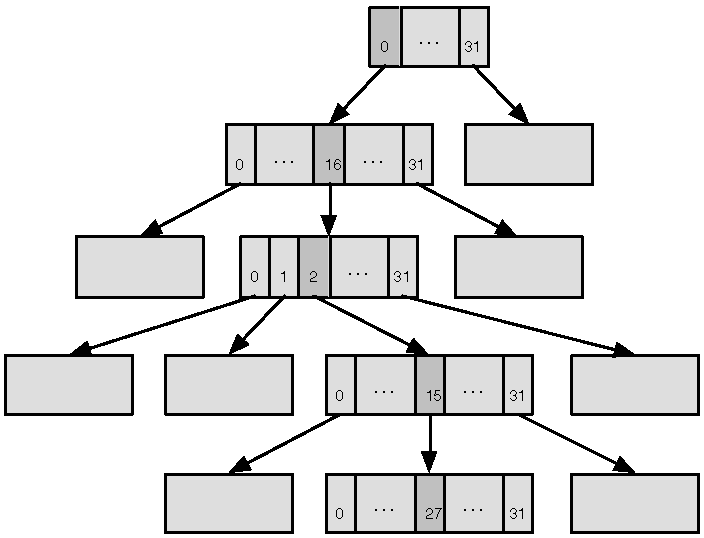
\includegraphics[width=0.5\textwidth]{Figures/Radix_Balanced_index_example}
  \caption{Accessing element at index 526843 in a tree of depth 5. Empty nodes represent collapses subtrees.}
  \label{radix_balanced_index_example}
\end{figure}

%-----------------------------------
%	SUBSECTION 3
%-----------------------------------

\subsection{Abstractions}
% function calls
% generic code vs specialized code


%----------------------------------------------------------------------------------------
%	SECTION - Displays
%----------------------------------------------------------------------------------------

\section{Displays}
% describe display fields in vector object
% describe the focus field

\begin{figure}[h!]
  \centering
  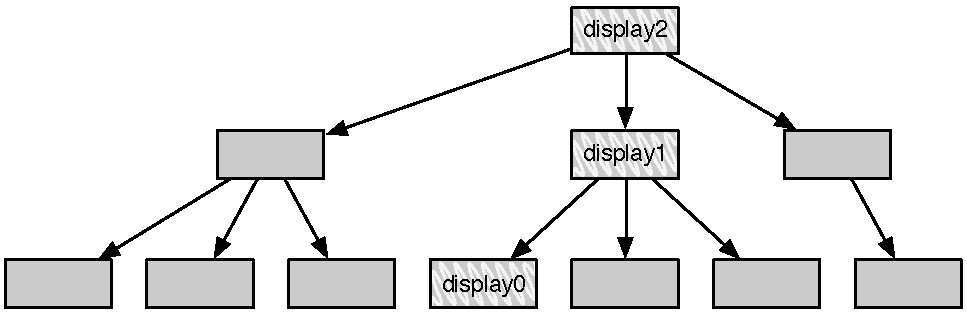
\includegraphics[width=\textwidth]{Figures/Displays}
  \label{Displays}
  \caption{Displays}
\end{figure}

%-----------------------------------
%	SUBSECTION As cache
%-----------------------------------

\subsection{As cache}
% used to access some elements directly from the smaller subtrees
% keeping relevant branch for next operations
% operations: all operations that involve the tree structure


%-----------------------------------
%	SUBSECTION  For transient states
%-----------------------------------

\subsection{For transient states}
% transient states are used to amortized operations
% operation: append, prepend, update

\begin{figure}[h!]
  \centering
  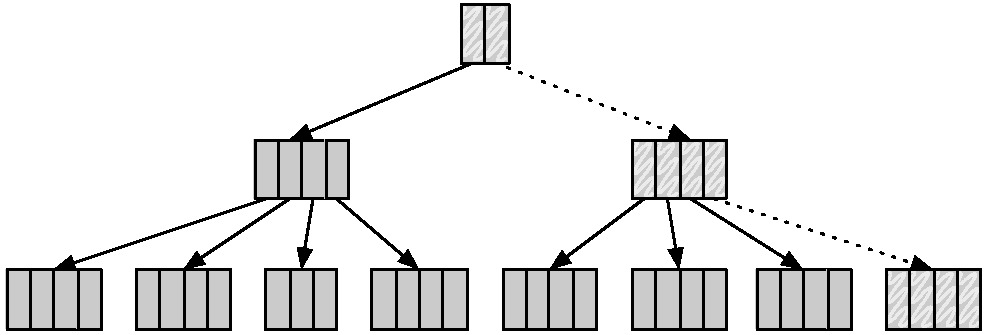
\includegraphics[width=\textwidth]{Figures/Transient_state}
  \label{Transient_state}
  \caption{Radix Balanced Tree Transient state}
\end{figure}


%----------------------------------------------------------------------------------------
%	SECTION - Builder
%----------------------------------------------------------------------------------------

\section{Builder}
% use of mutable tree 
% avoid creation unnecessary arrays



%----------------------------------------------------------------------------------------
%	SECTION - Iterator
%----------------------------------------------------------------------------------------

\section{Iterator}
% efficient tree traversal vs iteration by index
% avoid re-traversing vertically the tree from the root


%----------------------------------------------------------------------------------------
%	SECTION - Relaxing the radix
%----------------------------------------------------------------------------------------

\section{Relaxing the Radix}

%-----------------------------------
%	SUBSECTION Relaxing Displays
%-----------------------------------

\subsection{Relaxing Displays}
% describe fundamental difference in the focus (focused on balanced subtree)
% describe focus start, focus end and focus (focus relaxed)
% describe how fetching elements change

\begin{figure}[h!]
  \centering
  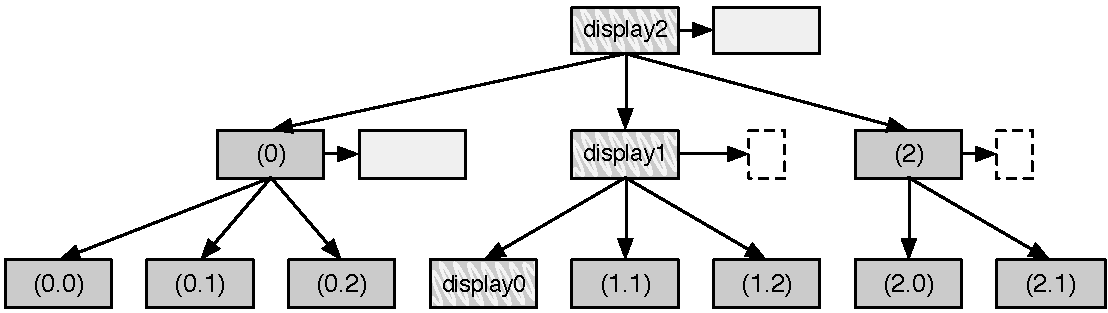
\includegraphics[width=\textwidth]{Figures/Balanced_subtrees}
  \label{Balanced_subtrees}
  \caption{Radix Balanced Tree}
\end{figure}

%-----------------------------------
%	SUBSECTION Displays
%-----------------------------------

\subsection{Relaxing the Builder}
% same base implementation for +=
% addition of accumulator for  ++= 

%-----------------------------------
%	SUBSECTION Displays
%-----------------------------------

\subsection{Relaxing Iterator}
% same implementation within a balanced subtree
% refocus from root to iterate between balanced subtrees



